\chapter{Fundamentação Teórica}


\section{Arquiteturas Paralelas}

De acordo com Tanenbaum~\etal~\cite{Tanenbaum2015}, as arquiteturas paralelas podem ser classificadas em
dois grandes grupos: multiprocessadores e multicomputadores. Nas seções a seguir são apresentados os
principais conceitos básicos destas duas classes de arquiteturas paralelas. Posteriormente, será discutido
em mais detalhes o processador \textit{manycore} \mppa, o qual será utilizado neste trabalho.

% \todo[inline]{Para o restante desta seção, tu podes pegar informações do livro do Tanenbaum de SO. O capítulo 8
% trata sobre multiprocessadores (seção 8.1) e multicomputadores (seção 8.2)}

\subsection{Multiprocessadores}

% \todo[inline]{
% - Organização: processadores interconectados a uma memória compartilhada via barramento (UMA). Podes usar a figura
% 8.2c do livro como base para fazer uma tua e mostrar as ideias.
% }

% \todo[inline]{
% - Podes falar rapidamente sobre NUMA e as diferenças para o UMA.
% }

% \todo[inline]{
% - Então, podes entrar no assunto dos multicores:

Multiprocessadores são sistemas que possuem uma ou mais \cpus que compartilham totalmente
a \ram do sistema. Desta forma, \textit{threads} de um mesmo processo se
comunicam através do mesmo espaço de endereçamento, por meio de escrita e
leitura na memória. Essa característica do sistema pode ocasionar problemas de
concorrência, onde um valor escrito por uma \textit{thread}, localizado em uma
palavra na memória, pode ser alterado por outra \textit{thread}, trazendo inconsistência no
sistema.

Mais especificamente, multiprocessadores podem possuir propriedades adicionais,
como acesso uniforme à memória. Máquinas com essa propriedade são chamadas de
\uma. Por outro lado, existem multiprocessadores que não apresetam essa
característica, como é o caso de multiprocessadores \numa, que apresentam um acesso
não-uniforme à memória.

A Figura~\ref{fig:uma} apresenta a arquitetura de sistemas multiprocessados \uma
mais simplificados, onde apresentam várias \cpus que se
comunicam com uma memória compartilhada por meio de um barramento. Quando uma
\cpu deseja efetuar a comunicação, o barramento é verificado para
determinar a sua disponibilidade. Caso o barramento esteja ocupado, a
\cpu espera até que ele fique livre. Com o barramento livre, a \cpu
coloca o endereço da palavra no barramento, utiliza sinais de
controle e espera até que a memória coloque esse endereço no barramento. Esse
método é gerenciável para poucas \cpus, contudo com uma maior quantidade, o
número de comunicações aumenta significativamente, tornando
o gerenciamento de comunicações por meio do barramento insuportável. Desta
forma, o barramento se torna o gargalo do sistema.

\begin{figure}[b]
	\centering
    \caption{Esquema genérico de um multiprocessador \uma.}
    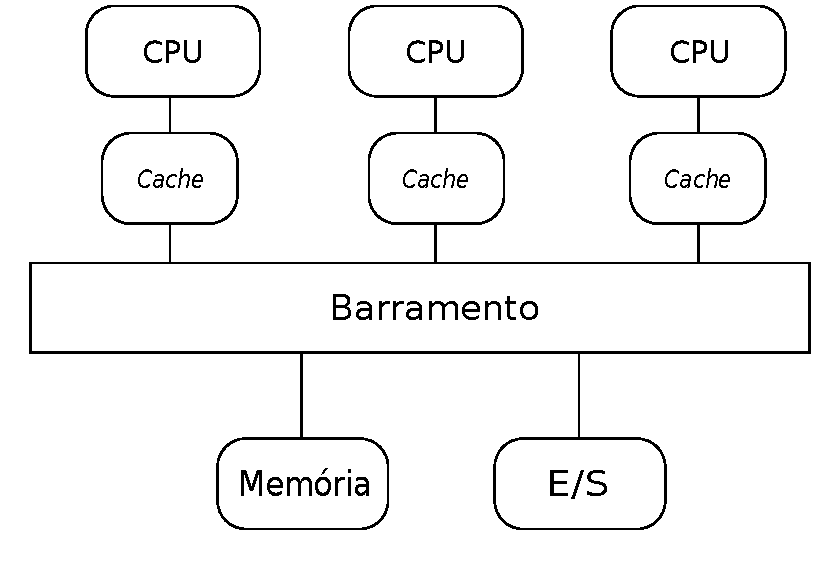
\includegraphics[width=0.6\textwidth]{figs/multiproc.pdf}
    \caption*{Fonte: desenvolvido pelo autor.}
    \label{fig:uma}
\end{figure}

\begin{figure}[b]
	\centering
    \caption{Esquema genérico de um multiprocessador \numa.}
    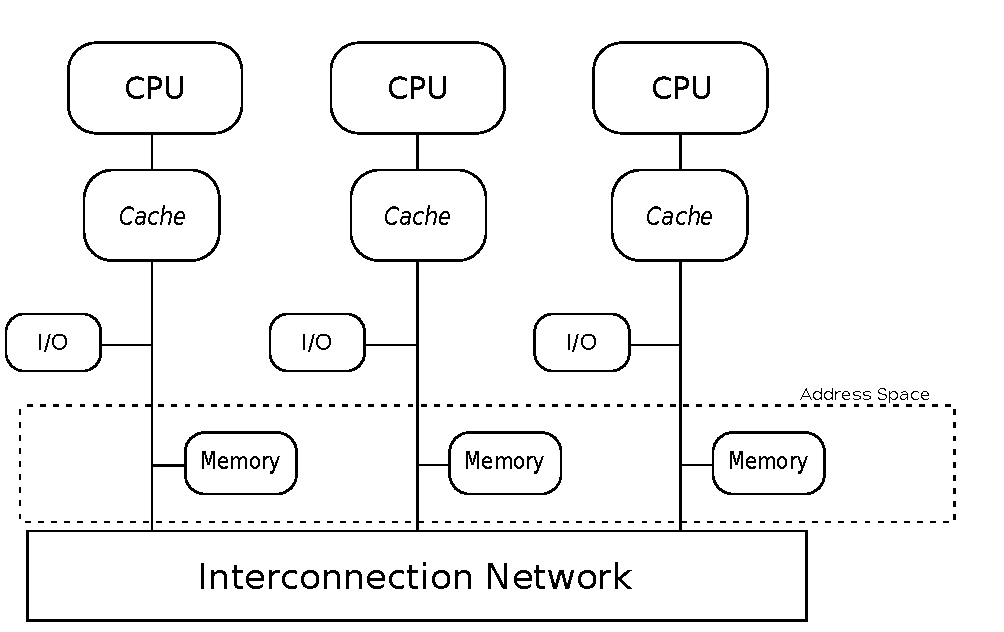
\includegraphics[width=0.7\textwidth]{figs/multiprocNUMA.pdf}
    \caption*{Fonte: desenvolvido pelo autor.}
    \label{fig:numa}
\end{figure}


A solução é utilizar \textit{caches} nas \cpus, desta forma, requisições
de leitura podem ser satisfeitas pela \textit{cache}, diminuindo a quantidade de
comunicações. É possível adicionar mais \cpus no barramento devido a baixa
quantidade de tráfego. \textit{Caches} possuem protocolos de coerência para
manter a consistência das \textit{caches} e do sistema. Quando uma \cpu
efetua uma escrita sobre uma palavra, todas as \textit{caches} que possuem essa
palavra serão notificadas. Uma \textit{cache} com uma cópia modificada, isto é,
diferente do dado presente na memória, deve escrever essa cópia diretamente na
memória. Caso uma cópia exata do dado na memória esteja presente na
\textit{cache}, ele pode ser descartado fazendo com que a \cpu acesse
diretamente a memória.

Além disso, é possível inserir mais \textit{caches} nas \cpus
diminuindo o tráfego, e retirando a necessidade de mais acessos à memória
principal. Contudo, devido ao limite arquitetural, uma quantidade muito grande
de \textit{caches} é inviável. Além disso, um tamanho muito grande para
\textit{caches} torna o seu acesso muito lento, prejudicando o desempenho do
sistema.

Sistemas multiprocessados \numa são diferentes de sistemas \uma, como mencionado
anteriormente, devido ao acesso à memória remota ser mais lento que à memória
local. A Figura~\ref{fig:numa} apresenta a arquitetura desse sistema, onde
existem nós interconectados por uma rede, e cada nó possui uma \cpu e um bloco
de memória. A \cpu de cada nó pode possuir uma \textit{cache}, possibilitando
uma redução no tempo de acesso à um dado localizado em uma memória remota, esse
sistema é denominada de \ccnuma. Por outro lado, um sistema sem \textit{cache} é
denominado \ncnuma.

Com o desenvolvimento de novas tecnologias, o tamanho
dos transistores diminuiu significativamente, se tornando possível inserir um
grande número de transistores em um único \textit{chip}.
Com o aumento da quantidade de transistores, um \textit{chip} pode ter, por
exemplo, várias \cpus, denominadas \textit{cores}, caracterizando um
\textit{chip} multicore.

Geralmente chamados de \cmps, os multicores são semelhantes à multiprocessadores
tradicionais, contudo, devido à proximidade de conexão entre \cpus, falhas em um
componente pode ocasionar problemas em outros componentes do sistema.

\soc é uma categoria de \textit{chips} multicores, onde existem uma ou mais
\cpus, e \textit{cores} de propósito específico, como decodificadores de áudio e
vídeo, interface de rede, entre outros.


Quando a quantidade de \textit{cores} é grande, isto é, dezenas até milhares de
\textit{cores}, o \textit{chip} pode ser classificado como \textit{manycore}.
Contudo, o limite para classificar um \textit{chip} em \textit{manycore} ou
\textit{multicore} é flexível. Geralmente, quando a perda de um ou dois
\textit{cores} é aceitável, temos um \textit{manycore}~\cite{Tanenbaum2015}.
Atualmente, aceleradores com uma grande quantidade \textit{cores} estão
surgindo, como o Xeon Phi da Intel com 60 \textit{cores}.

Com vários \textit{cores} em um único \textit{chip} problemas de coerência de
\textit{cache} começam a surgir. Mais especificamente, com o aumento no número
de \textit{cores}, o custo sobre o protocolo de coerência vai crescer até que
aumentar o número de \textit{cores} não auxiliará mais o desempenho, pois o sistema
estará gastando muito tempo mantendo as \textit{caches} consistentes.


Atualmente, sistemas computacionais comuns apresentam uma \gpu, onde temos
milhares de \textit{cores} disponíveis. \gpus utilizam esses \textit{cores},
essencialmente, para a solução de cálculos, focando menos em questões de
\textit{cache} e lógica de controle. Desta forma, elas são utilizadas em
pequenas computações que podem ser paralelizadas. Contudo, a programação para
\gpus é difícil, pois os seus \textit{cores} fazem a execução da mesma intrução
com diferentes partes do dado, isto é, são máquinas \simd. Esse modelo de
programação é interessante para abordar o paralelismo de dados, contudo, o
desenvolvedor pode se deparar com dificuldades durante o desenvolvimento para
essa máquina. Desta forma, linguagens de programação, como CUDA e \opengl,
abstraem o desenvolvimento de aplicações para esses sistemas computacionais.

O \mppa é um processador \textit{manycore} diferente dos apresentados acima,
pois os seus \textit{cores} são conectados atraves de uma \noc. Mais detalhes
sobre esse assunto serão tratados na seção 2.1.3.

% Até a última década, o desempenho sobre computadores escalava de acordo com o
% aumento da frequência dos processadores.
%
%
% Contudo, com o aumento da frequência,
% a potência e o consumo de energia também aumentam. De acordo com a
% Equação~\eqref{eq:power}, pode-se perceber que a potência aumenta,
% proporcionalmente, com o aumento da frequência.
%
%
% \begin{equation}\label{eq:power}
% 	P = CV^2f
% \end{equation}
%
% \todo[inline]{Esta parte está ruim. 1) Não foi explicada a equação (o que é P, C, V e f?).
% 2) Dizer que a potência aumenta proporcionalmente com o aumento da frequência não está totalmente correto,
% pois a tensão (V) também tem relação com a frequência (f). A tensão tem um impacto ainda maior, pois
% ela é quadrática na equação. Tens que dar uma olhada melhor nisso e corrigir o texto.}
%
% Portanto, o aumento do desempenho encontrou uma barreira no consumo de energia, onde tornou-se inviável
% um aumento indiscriminado da frequência. Desta forma, tornou-se necessário uma
% nova abordagem para aumentar o desempenho dos processadores. A solução encontrada
% pelos fabricantes de \textit{chips} foi de aumentar a quantidade de núcleos processamento no \textit{chip},
% porém reduzindo a frequência de operação dos mesmos, dando origem aos processadores \textit{multicore}.
%
% \todo[inline]{
% - Falar de \textit{manycores} (de modo geral), dando exemplos: Xeon Phi e GPU, que são dois tipos de \textit{manycores}
% bem diferentes.
% }
%
% \todo[inline]{
% - Finalizar dizendo que o \textit{manycore} utilizado neste trabalho se diferencia dos dois exemplos anteriores, pois
% seus núcleos são conectados através de uma NoC. Então, diz que será tratado desse assunto na Seção 2.1.3
% }
%
\subsection{Multicomputadores}

% \todo[inline]{
% - Organização: sistemas multiprocessados, cada um com sua memória de dedicada, conectados através de uma rede. Podes usar
% a figura 8-18 como base para explicar as ideias.
% }
%
% \todo[inline]{
% - Podes falar rapidamente dos diferentes tipos de interconexão: figura 8-16 do livro
% }
%
% \todo[inline]{
% - Falar dos tipos de multicomputadores: NOW, COW, etc...
% }
%
% \todo[inline]{
% - Finalizar indicando que nos multicomputadores a comunicação entre os processadores é feita de maneira explícita através de trocas de mensagens.
% }
%
Multiprocessadores de grande porte são difíceis de construir devido ao alto
custo. Desta forma, devido a simplicidade de construção, multicomputadores
começaram a surgir, que utilizam \cpus fortemente aclopadas sem compartilhamento
de memória~\cite{Tanenbaum2015}. Um \pc comum e uma placa de interface de rede formam um nó do
sistema multicomputado, onde um gerenciamento de forma inteligente a rede auxilia o desempenho
do sistema.

\begin{figure}[t]
	\centering
    \caption{Esquema simples de um sistema multicomputado.}
        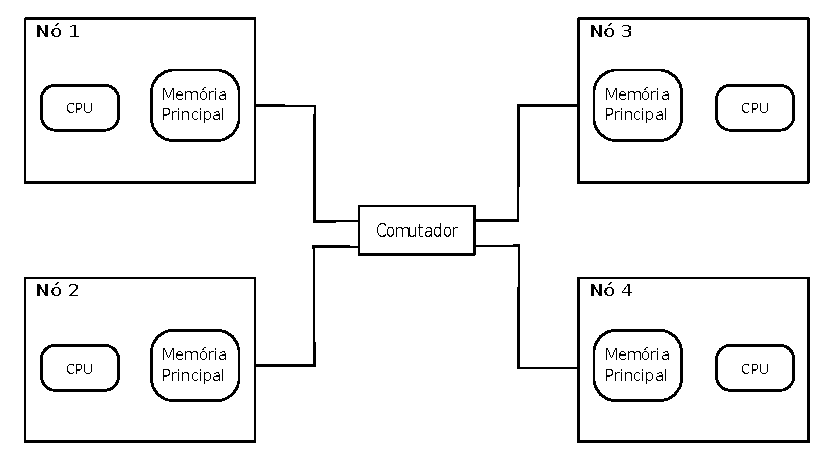
\includegraphics[width=0.7\textwidth]{figs/multicomp.pdf}
        \caption*{Fonte: desenvolvido pelo autor.}
        \label{fig:multicomputado}
\end{figure}



A Figura~\ref{fig:multicomputado} mostra como um sistema multicomputado simples é
organizado. Existem nós que possuem uma \cpu, memória principal dedicada e uma
conexão diretamente com outros nós ou à um comutador. A topologia apresentada na
imagem é uma das topologias possíveis em um sistema multicomputado. Outra
alternativa é utilizar uma topologia em anel, retirando a necessidade de um
comutador, pois um nó é conectado diretamente aos outros nós. Cada nó é
conectado ao nó à sua esquerda e à sua direita.

Topologia em malha (\textit{mesh}) da Figura~\ref{fig:topologia}c conecta os nós
em comutadores distindos pelo sistema, e cada comutador conectado à outros
comutadores, formando uma espécie de malha no sistema. Uma variante dessa
topologia é o toro duplo apresentado na Figura ~\ref{fig:topologia}d, onde os
comutadores de cantos opostos estão conectados diretamente. Desta forma, a
comunicação entre nós de cantos opostos não terão a necessidade de inúmeros
saltos pelos comutadores para efetuar a transmissão de informações.

A Figura~\ref{fig:topologia}e ilustra uma topologia tridimensional, e a
Figura~\ref{fig:topologia}f ilustra um cubo tetradimensional. Topologias
$n$ dimensionais são utilizadas para diminuir o atraso de comunicação entre nós,
pois o diâmetro da rede cresce linearmente de acordo com a dimensionalidade.
Devido à essa propriedade, topologias $n$ dimensionais são utilizadas em
computadores paralelos.




\begin{figure}[t]
	\centering
        \caption{Topologias de interconexão.}
	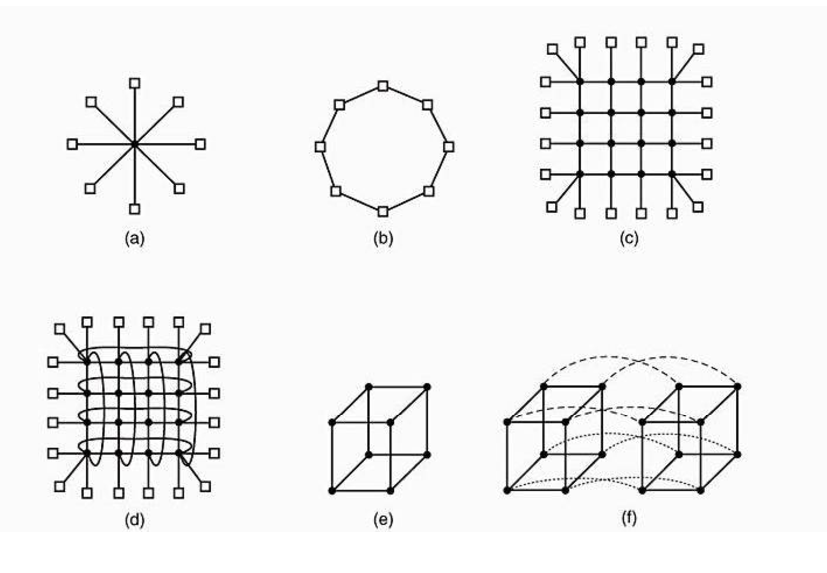
\includegraphics[width=\textwidth]{figs/topologia.pdf}
    \caption*{Fonte: \cite{Tanenbaum2015}}
    \label{fig:topologia}
\end{figure}


%Cow Now
Geralmente, multicomputadores podem ser construídos com computadores pessoais
comuns interconectados por uma \textit{interface} de rede para trabalharem em
conjunto sobre uma operação, esse sistema é denominado de \now. Devido à sua
simplicidade, esse sistema não é focado em ganho de desempenho. \cow
são constituídos de computadores interconectados sem teclado, monitor e \textit{mouse}. Esses
sistemas são focados em desempenho, subdividindo tarefas e enviando por meio de
uma conexão eficiênte para ganhar o máximo em desempenho sobre uma operação.

A comunicação em um multicomputador é feita por meio de troca de mensagens.
Processos localizados em diferentes \cpus se comunicam por meio de operações
disponibilizadas pelo \so. Mais especificamente, o \so disponibiliza, pelo
menos, duas chamadas de função: \textit{send} e  \textit{recieve}. Na função
\textit{send} o desenvolvedor envia uma mensagem para um processo determinado pelos
parâmetros da função. A função \textit{recieve} é responsável pelo recebimento
de mensagens, utlizando como parâmetro o endereço que será lido para coletar a
mensagem recebida. Portanto, em sistemas multicomputados a troca de mensagens
entre processos é realizada de maneira explícita pelo desenvolvedor.


\subsection{O Processador \textit{Manycore} MPPA-256}

O \mppa é um processador \textit{manycore} desenvolvido pela empresa francesa
Kalray, o qual possui 256 núcleos de processamento de 400 MHz. Ele mistura características
de um multiprocessador e de um multicomputador, porém em um único \textit{chip}.
Mais especificamente, o \mppa utiliza um modelo multicomputado com uma
comunicação via \noc em seus \textit{clusters}, e um modelo multiprocessado
dentro de cada \textit{cluster}.

Os núcleos de processamento do \mppa são denominados \pes.
Além dos \pes, o processador possui 32 núcleos dedicados a gerência de recursos
denominados  \rmans. \pes e \rmans são distribuídos
fisicamente no \textit{chip} em 16 \textit{clusters} e 4 subsistemas de \es,
contendo cada \textit{cluster} 16 \pes e 1 \rman. Além dos \textit{clusters}, o
\mppa possui 4 subsistemas de \es contendo, cada um, 4 \rmans. Toda a comunicação
entre \textit{clusters} e/ou subsistemas de \es é feita através de uma \noc
\textit{torus} 2D. A arquitetura do \mppa pode ser vista na Figura~\ref{fig:mppa}.

A finalidade principal dos \pes é executar \textit{threads} de usuário de forma
ininterrupta e não preemptível para realização de computação. \pes de um mesmo
\textit{cluster} compartilham uma memória de 2~\mb, a qual é utilizada para
armazenar os dados a serem processados pelos \pes. Cada \pe possui também uma
memória \textit{cache} associativa 2-\textit{way} de 32~\kb para dados e uma para
instruções. Porém, o processador não dispõe de coerência de \textit{caches}, o
que dificulta o desenvolvimento de aplicações para esse processador. Por outro
lado, a finalidade dos \rmans é gerenciar \es, controlar comunicações entre
\textit{clusters} e/ou subsistemas de \es e realizar comunicação com uma memória
\ram. Na arquitetura utilizada, um dos subsistemas de \es está conectado a uma
memória externa \lpddr de 2~\gb.

\begin{figure}
	\centering
	\caption{Visão geral do \mppa.}
	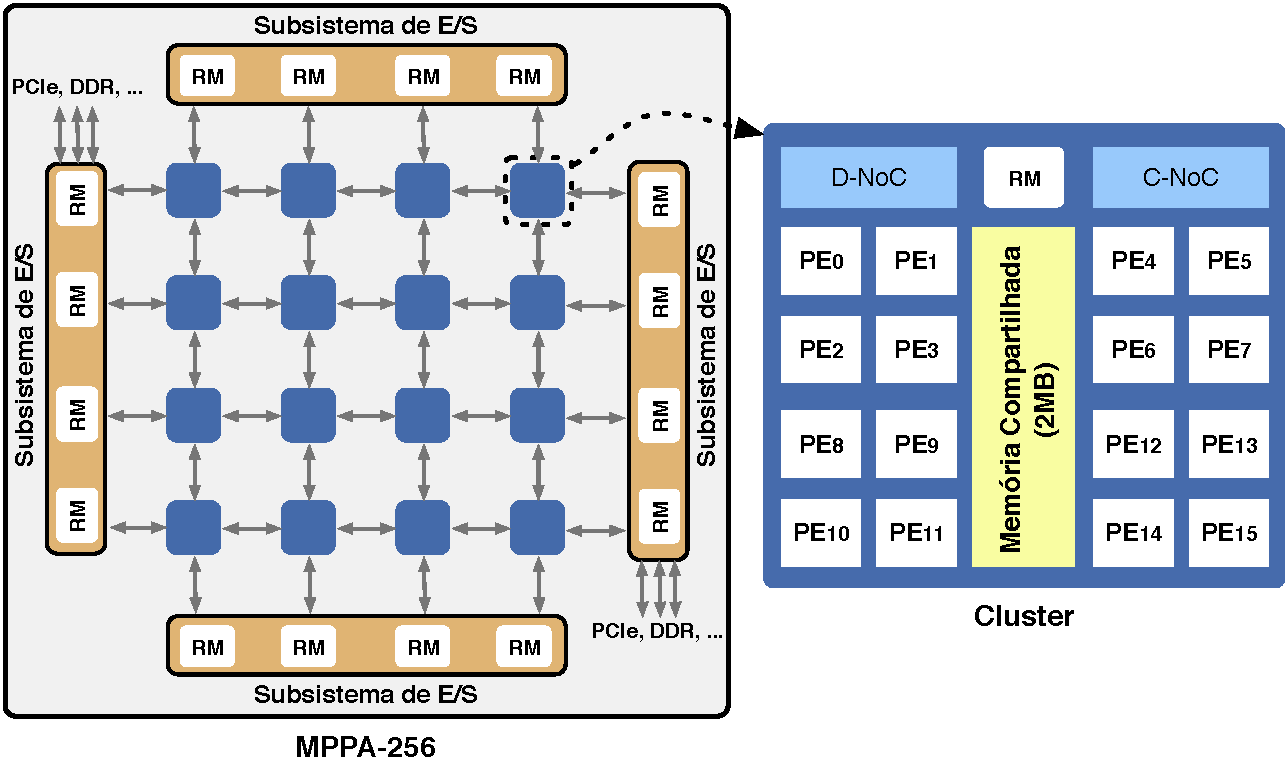
\includegraphics[width=0.7\textwidth]{figs/mppa-overall.pdf}
    \caption*{Fonte: ~\cite{Castro-IA3:2013}}
	\label{fig:mppa}
\end{figure}

A comunicação dos \textit{clusters} com o subsistema de \es, e a comunicação
entre \textit{clusters} é realizada de maneira explícita, utilizando uma \api
própria do \mppa de baixo nível similar à \posix \ipc. Detalhes referentes à
essa comunicação e programação nesse processador serão abordads na seção
2.2.3.

% - Terminar essa seção falando que a comunicação entre clusters e entre cluster/IO tem
% que ser feita de maneira explícita utilizando uma API de baixo nível. Então, diz que os detalhes
% referentes a programação nesse processador serão tratados na Seção 2.2.3
%----------------------------------------------------------------------------------------
%Existem diversos tipos de arquiteturas que proporcionam ao desenvolvedor uma
%abordagem paralela. Multiprocessadores são arquiteturas que fornecem vários
%núcleos de processamento em uma máquina e a comunicação entre os núcleos é feita
%através da memória compartilhada, contudo este modelo traz dificuldades em
%relação à organização e particionamento de dados entre núcleos. Devido ao espaço
%limitado em \textit{chip}, o aumento do número de núcleos nessa arquitetura pode
%se tornar inviável, portanto, arquiteturas multicomputadas são utilizadas, onde
%temos várias máquinas, sendo, geralmente, multiprocessadas, interligadas para
%fornecer um maior poder de processamento. A comunicação entre cada
%\textit{cluster}, isto é, cada nó na rede de computadores utiliza distribuição
%de dados e sincronizações, como não temos compartilhamento de memória entre os
%nós de processamento, o desenvolvimento de código para essa arquitetura é mais
%complicada, pois existem vários fatores à serem avaliados pelo desenvolvedor. Na
%próxima seção serão abordadas as dificuldades e implementação de cada modelo.

%Arquiteturas paralelas: multicomputadores, multiprocessadores, compartilhamento de memória e distribuição de dados.
%Programação paralela: uso de apis, dificuldades. POSIX, MPI...


\section{Programação Paralela}

O desenvolvimento de aplicações são, geralmente, implementadas de forma
sequencial, isto é, um conjunto serializado de instruções que será executado
sobre uma \cpu. Por outro lado, a computação paralela ou distribuída efetua o
processamento de instruções sobre múltiplos elementos de processamento. A ideia
principal é dividir a computação em partes menores que podem ser executadas
simultaneamente entre os elementos de processamento distintos com intuito de se
realizar um processamento em menos tempo.

Diferentes APIs de programação paralela foram criadas com intuito de simplificar
o desenvolvimento de aplicações em arquiteturas multiprocessadas e multicomputadas.
A seguir, serão apresentadas as APIs mais utilizadas no âmbito de \hpc em cada tipo de
arquitetura. Por fim, será apresentada a \api utilizada para o desenvolvimento de aplicações
no processador \mppa.


\subsection{OpenMP}

% \todo[inline]{
% - Dizer que é feita para ser utilizada em arquiteturas multiprocessadas, ou seja, com memória
% compartilhada.
% }
%
% \todo[inline]{
% - Apresentar as principais ideias do OpenMP: dizer que é baseada em pragmas, modelo fork-join,
% regiões paralelas, paralelização de laços, ... (A \api é baseada no modelo de programação
% paralela de memória compartilhada, apresentando uma boa portabilidade e pouco
% esforço de programação. O modelo de programação utiliza diretivas de compilação
% e variáveis, tornando possível poucas modificações de código para utilizar
% outras \textit{threads} na aplicação....)
% }


Para evitar uma programação de baixo nível sobre um sistema multiprocessado, são
utilizadas \apis para o desenvolvimento de aplicações, como o OpenMP. O OpenMP
é um modelo de programação baseado em memória compartilhada, e apresenta boa
portabilidade, um bom desempenho e escalabilidade. Devido à abstração que a \api
fornece, o desenvolvimento de aplicações para o ambiente multiprocessado é
facilitado, permitindo paralelização de aplicações com variáveis de ambiente e
diretivas de compilação.

O OpenMP utiliza o modelo \textit{fork-join}, onde a execução inicia com uma
única \textit{thread}, denominada \textit{master thread}. Como ilustrado na
Figura~\ref{fig:forkjoin}, quando a \textit{master thread} encontra
uma região paralela, são criadas outras \textit{threads} de acordo com a variável
de ambiente especificada no sistema. No final da região paralela, é realizado um
\textit{join} por meio de uma barreira implícita, onde as \textit{threads} serão
sincronizadas, e a execução irá continuar apenas com a \textit{master thread}.

\begin{figure}
	\centering
	\caption{Esquemático do modelo \textit{fork-join}.}
	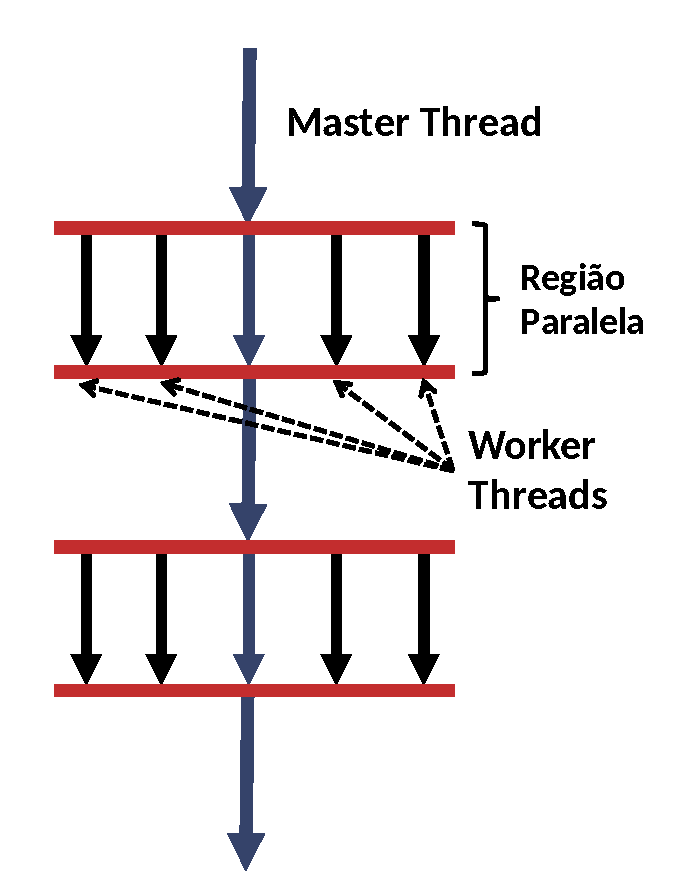
\includegraphics[width=0.4\textwidth]{figs/forkjoin.pdf}
    \caption*{Fonte: desenvolvido pelo autor}
	\label{fig:forkjoin}
\end{figure}

Por meio de diretivas de compilação é possível definir o comportamento do
OpenMP, inclusive determinar regiões paralelas, entre outras funções da \api.
Dados são classificados em \textit{shared} ou \textit{private} possibilitando
o gerenciamento da execução pela \api. Um dado \textit{shared} é compartilhado
entre as \textit{threads} de uma região paralela. Por outro lado, dados
\textit{private} são privados para cada \textit{thread}, isto é, possuem uma
cópia do dado. Desta forma, as modificações sobre os dados é local em cada
\textit{thread}.

As diretivas do OpenMP, além de determinar regiões paralelas, possibilitam
paralelizar \textit{loops} de maneira automática, onde as iterações
do \textit{loop} são distribuídas, de forma automática e flexível, sobre as
\textit{threads} da região paralela. Além disso, operações de redução podem ser
utilizadas ao fim de uma região paralela, aplicando sobre uma variável a
operação especificada. Ao final da região paralela, o resultado é atribuído à
uma variável compartilhada.

Devido à abstração que o modelo oferece, poucas modificações de código são
necessárias para paralelizar uma aplicação. \posix \textit{threads} é outro
modelo que pode ser utilizado, contudo com uma menor abstração que o modelo
OpenMP.

%Computação paralela em uma arquitetura multiprocessada contém diversas
%dificuldades para o desenvolvimento de código, como: \textbf{(i) dependência de
%    dados:} quando um processo ou \textit{thread} está executando uma parte do
%código, outra \textit{thread} deve ter os dados atualizados corretamente. Esta
%dependência pode gerar problemas, como \textit{deadlocks} e \textit{livelocks}.
%\textit{Deadlocks} são conflitos que ocorrem entre \textit{threads}, quando uma
%\textit{thread} $A$ precisa de um recurso alocado por uma \textit{thread} $B$
%que, por sua vez, precisa de um recurso alocado pela \textit{thread} $A$, ocorre
%um ciclo na execução, caracterizando um \textit{deadlock}. Por outro lado,
%\textit{Livelocks} são similares aos \textit{deadlocks}, contudo o estado das
%\textit{threads} estão em constante mudança, fazendo com que nenhum deles
%continue sua execução normalmente, pois a cada mudança um \textit{deadlock}
%ocorre. Além disso, dependências geram problemas de sincronização entre
%\textit{threads}, deixando para o desenvolvedor da aplicação a tarefa de
%gerenciar corretamente a execução. \textbf{(ii) Condição de Corrida:} uma
%\textit{thread} escreve sobre uma váriavel ou, mais especificamente, um espaço
%de memória, enquanto outra \textit{thread} fará alguma operação sobre esse mesmo
%espaço. Isso pode gerar inconsistências de dados, entre outros problemas.

\subsection{MPI}

% \todo[inline]{
% - Motivação para usar MPI:
%
% A programação paralela em multicomputadores é feita através da utilização de múltiplos processos que se comunicam
% através de trocas de mensagens. Devido à característica de baixo nível intrínseca do modelo de troca de
% mensagens, utilizar \textit{sockets} manualmente para a comunicação entre nós de
% uma rede de \textit{clusters} é inadequada para o desenvolvedor. Portanto, mostra-se necessário utilizar
% APIs de mais alto nível, possibilitando uma maior abstração ao desenvolvedor.
% }
%
% \todo[inline]{
% - Dizer que MPI é a API mais amplamente utilizada para programação paralela em multicomputadores, ou seja, para arquiteturas multicomputadas, ou seja, com memória distribuída.
% }
%
% \todo[inline]{
% - Apresentar as principais ideias do MPI: processos MPI, rank, Send/Recv, comunicações coletivas, ...
% }

A programação paralela em multicomputadores é feita através da utilização de múltiplos processos que se comunicam
através de trocas de mensagens. Devido à característica de baixo nível intrínseca do modelo de troca de
mensagens, utilizar \textit{sockets} manualmente para a comunicação entre nós de
uma rede de \textit{clusters} é inadequada para o desenvolvedor. Portanto, mostra-se necessário utilizar
APIs de mais alto nível, possibilitando uma maior abstração ao desenvolvedor.

O \mpi é uma \api utilizada amplamente em multicomputadores fornecendo uma maior
abstração em relação à programação sobre \textit{sockets}. A \api é baseada no
modelo \spmd, onde todos os processos executam o mesmo código fonte com
dados diferentes. Desta forma, com apenas um código fonte, processos diferentes
serão responsáveis por realizar diferentes operações, fornecendo uma abordagem
paralela sobre código.

A \api utiliza funções, como \texttt{MPI\_Init} para inicializar a alocação de
\textit{buffers} e  especificar um inteiro positivo para cada processo. Esse
inteiro positivo, denominado \textit{rank}, será responsável por determinar qual
processo será selecionado para um envio ou recebimento de uma mensagem, por
exemplo. Para finalizar o uso do \mpi e liberar as alocações realizadas, é feita
uma chamada para a função \texttt{MPI\_Finalize}. O envio de mensagens pela \api
é realizada pela função \texttt{MPI\_Send}, que construirá a mensagem, e irá
adicionar o \textit{rank} do destinatário, o \textit{rank} do remetente, entre
outras informações. A função \texttt{MPI\_Recv} será responsável por receber a
mensagem enviada pelo processo, e irá armazená-la no espaço de memória
do processo destinatário.

Além de comunicações entre dois processos, existem comunicações coletivas entre
todos os processos. Funções como \texttt{MPI\_Barrier} e \texttt{MPI\_Bcast} são
utilizadas para informar todos os processos do sistema. A função
\texttt{MPI\_Barrier} é uma barreira de sincronização, responsável por bloquear a
execução de um processo até que todos os outros processos cheguem na barreira.
Por outro lado, a função \texttt{MPI\_Bcast} é responsável por enviar a mesma
mensagem de um processo para todos os outros processos do sistema.

%
% \renewcommand{\lstlistingname}{Código}
% \definecolor{lightgray}{rgb}{0.97,0.97,0.97}
% \definecolor{lightred}{rgb}{1,0.7,0.7}
%
% \lstdefinelanguage{cc}{
%     language     = C++,
%     morekeywords = {Array2D, __parallel__, Mask2D, Stencil2D, pragma, omp, parallel, printf},
% }
%
% \lstset{
% numbers=none,
% stepnumber=1,
% numbersep=-8pt,
% numberstyle=\small\color{black},
% basicstyle=\scriptsize\ttfamily,
% keywordstyle=\color{blue},
% commentstyle=\color{black},
% stringstyle=\color{black},
% numberstyle=\footnotesize\ttfamily\color{black},
% escapeinside={(@}{@)},
% frame=none, %single
% tabsize=2,
% float,
% language=cc, %morecomment=[l][{\color[rgb]{0.1, 0.2, 0.8}}]{},
% %aboveskip=0.1in, % space before the caption
% %belowskip=0.1in, % space after listing
% captionpos=b,
% showstringspaces=false,
% %belowcaptionskip=1\baselineskip,
% %breaklines=true,
% %moredelim=[l][\color{blue}]{\#pragma},
% backgroundcolor=\color{white},
% %xleftmargin=.2\textwidth, xrightmargin=.2\textwidth
% }
%
% \begin{figure}[thp] % the figure provides the caption
% \centering          % which should be centered
% \begin{tabular}{c}
%
% \begin{lstlisting}[]
%     (@\textcolor{blue}{\#}@)pragma omp parallel
%     printf("Hello World!");
% \end{lstlisting}
% \end{tabular}
% \caption*{Exemplo de código OpenMP.}
% \end{figure}
%
% \todo{Apresentar código \MPI}


%Ao aperfeiçoar esses modelos, começaram a surgir processadores para \hpc com
%vários \textit{cores} de processamento. Esses processadores utilizam várias
%técnicas, que abordam o paralelismo e características específicas de cada
%máquina, para aumentar o desempenho de aplicações. Com o aumento da importância
%do consumo de energia, novos porcessadores \textit{manycore} de baixo consumo de
%energia começaram a surgir. Contudo, processadores \textit{manycore} são
%onerosos e suceptíveis à erros, apresentando diversos problemas para o
%desenvolvedor~\cite{pereira15}. Geralmente, núcleos de processamento sem
%coerência de \textit{cache} são distribuídos em uma arquitetura organizada em
%\textit{clusters}, onde cada \textit{cluster} possui uma memória local
%(compartilhada somente entre os \textit{cores} do \textit{cluster}). Dessa
%forma, a comunicação entre \textit{clusters} deve ser feita de uma forma
%distribuída e a comunicação intra-\textit{cluster} deve ser feita por meio do
%modelo de memória compartilhada. Devido à comunicação entre os \textit{clusters}
%o peso do tempo de comunicação pode ter um grande impacto no tempo total de
%execução.
%-------------------------------------------------------------------

\subsection{Modelo de Programação do MPPA-256}

% \todo[inline]{
% - Falar de como se programa o MPPA: processo mestre roda no I/O, ele faz spawn de um
% processo escravo para cada cluster, cada processo escravo pode criar até 16 threads.
% }
%
% \todo[inline]{
% - Threads podem ser criadas usando POSIX ou OpenMP (que foi tratado anteriormente)
% }
%
% \todo[inline]{
% - Explicar que MPPA não tem suporte para a API MPI. Portanto, é necessário utilizar uma API de comunicação low-level
% desenvolvida pela Kalray. Explicar que cada  cluster tem seu espaço de endereçamento, que se usa o conceito de portais, para se
% fazer escrita remota, etc... Falar um pouco de como funciona essas comunicações através da NoC.
% }
%
% \todo[inline]{
% - Finaliza falando das dificuldades de se programar com essa API low-level (texto abaixo):
% }

O \mppa possui uma arquitetura interessante para um modelo mestre/trabalhador ou
um modelo \textit{pipeline} sobre os algoritmos. Desta forma, o processo mestre
é executado em um \rman no subsistema de \es, e é responsável por inicializar os
processos trabalhadores. Os processos trabalhadores são executados nos
\textit{clusters}, podendo criaraté 16 POSIX \textit{threads}, uma para cada \pe.

A Figura~\ref{fig:MPPAIPCTutorial} ilustra o funcionamento do modelo mestre e
escravo no \mppa. O processo mestre será responsável por iniciar os
\textit{clusters} por meio de uma função \texttt{spawn}, enviar dados e coletar
o resultado final. Por outro lado, o processo trabalhador recebe um dado e
realiza a computação utilizando \textit{threads}, que são criadas por meio da
\api OpenMP ou \posix. Após o processo trabalhador finalizar a computação sobre
um dado, ele irá enviar o resultado ao mestre.

O \mppa não possui suporte para o \mpi, desta forma, os processos mestre e
trabalhador utilizam objetos de comunicação, como portais e sincronizações, de
uma \api proprietária de baixo nível do \mppa, similar a \posix \ipc.

Devido à cada processo trabalhador possuir um espaço de endereçamento, são
utilizados portais para efetuar a comunicação entre o mestre e o trabalhador. Os
portais efetuam escrita e leitura remota, onde um processo deve criar um portal
com uma classificação, denominada \textit{tag}, e um
espaço de endereçamento para realizar a comunicação.

Para efetuar a escrita em um espaço de endereçamento é necessário chamar uma
função denominada \texttt{mppa\_pwrite}. Essa função utiliza como parâmetros o
portal que será utilizado na comunicação e o tamanho do dado que será enviado.
A função \texttt{mppa\_aio\_read} realizará a leitura dos dados recebidos pelo
portal, relacionando o portal que será feita a leitura com o espaço de
endereçamento em que o dado será armazenado.

\begin{figure}
	\centering
	\caption{Esquemático do modelo mestre/trabalhador no \mppa.}
	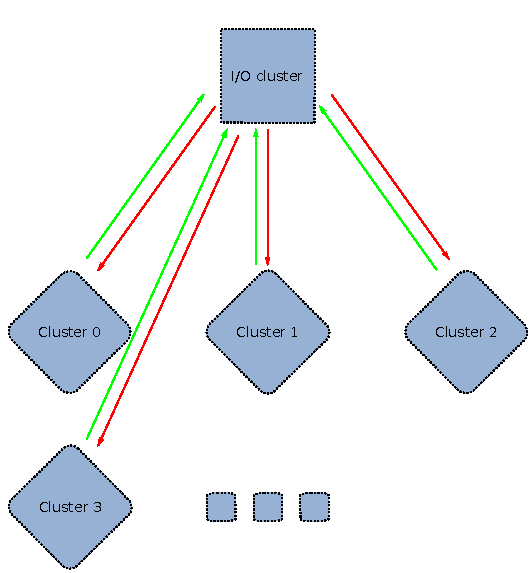
\includegraphics[width=0.5\textwidth]{figs/MPPAIPCTutorial.pdf}
    \caption*{Fonte: Manual do \mppa}
	\label{fig:MPPAIPCTutorial}
\end{figure}


O desenvolvedor de aplicações terá que desenvolver dois
códigos, um código para o mestre e outro para o trabalhador. O binário de cada
código será atribuído ao subsistema de \es ou ao \textit{cluster}, criando os
processos mestre e trabalhador.

Trabalhos anteriores mostraram que desenvolver aplicações paralelas otimizadas
para o \mppa é um grande desafio~\cite{Castro-IA3-JPDC:2014} devido a alguns
fatores importantes. O primeiro deles está relacionado ao \textbf{modelo de
    programação híbrido} exigido pelo processador: \textit{threads} em um mesmo
\textit{cluster} se comunicam através de uma memória compartilhada local, porém
a comunicação entre \textit{clusters} é feita explicitamente via \noc, em um
modelo de memória distribuída. Mais especificamente, aplicações desenvolvidas
para o \mppa precisam utilizar duas bibliotecas de programação paralela para
utilizar os recursos do processador: OpenMP, baseado em um modelo de memória
compartilhada, utilizada para paralelizar a computação dentro de cada
\textit{cluster} e uma \api proprietária, que segue um modelo de memória
distribuída, sendo utilizado na comunicação entre os \textit{clusters} e o
subsistema de E/S por meio da NoC. O segundo fator importante está relacionado a
\textbf{capacidade limitada de memória} no \textit{chip}: cada \textit{cluster}
possui apenas 2 MB de memória local de baixa latência. Portanto, aplicações
reais precisam constantemente realizar comunicações com o subsistema de \io
conectado à memória \lpddr. Por fim, o último fator está diretamente relacionado
à \textbf{ausência de coerência de \textit{cache}}: cada \pe possui uma memória
\textit{cache} privada sem coerência de \textit{cache}, sendo necessário o uso
explícito de instruções do tipo \textit{flush} para atualizar a \textit{cache}
de um \pe quando necessário.


\section{O Padrão \textit{Stencil}}

As dificuldades presentes na computação paralela tem um grande impacto sobre a
eficiência do desenvolvimento de aplicações para esse modelo. Com o
desenvolvimento de aplicações paralelas, começou-se a notar um padrão entre
elas. Com isso, foram criados os padrões paralelos para simplificar o
desenvolvimento de código.
% ~\cite{Cole M. Algorithmic skeletons: structured management of parallel computations, Research monographs in parallel and distributed computing.
% London: Pitman; 1989.}
% McCool MD. Structured parallel programming with deterministic patterns. Proceedings of the 2Nd USENIX Conference on Hot Topics in Parallelism, HotPar'10, USENIX Association, Berkeley, CA, 2010; 5–5.
Para uma maior abstração e redução da complexidade dos padrões, foram utilizados
esqueletos paralelos (\textit{skeletons}) O esqueleto será responsável por
gerenciar o controle de tarefas e dados, retirando essa responsabilidade do
desenvolvedor. Desta forma, é possível simplificar grande parte do
desenvolvimento de aplicações paralelas e auxiliar em outras funções que podem
trazer uma maior dificuldade ao desenvolvedor. Mais especificamente, o
desenvolvedor irá focar apenas em especificar o algoritmo, deixando o esqueleto
gerenciar os detalhes de execução, diminuindo o tempo de desenvolvimento e
\textit{debug} da aplicação.

Existem diversos padrões paralelos, como o \textit{map}, \textit{reduce},
\textit{scan}, \textit{stencil}, entre outros. Dentre os padrões existentes, o
padrão \textit{stencil} é de grande importância tanto no ambiente acadêmico quanto no
industrial, utilizado em diversos campos importantes, como física quântica,
previsão do tempo e processamento de imagens.~\cite{pereira15}.

O padrão \textit{stencil} atualiza elementos de uma matriz (\texttt{Array}) de entrada,
de acordo com um padrão especificado. Mais especificamente, em uma aplicação
\textit{stencil}, cada iteração utiliza a máscara de vizinhança (\texttt{Mask})
responsável por determinar os vizinhos utilizados na computação. A máscara é
aplicada sobre o \texttt{Array} de entrada para determinar o valor de cada
célula do \texttt{Array} de saída. No exemplo da Figura~\ref{fig:stencil}, o
valor de cada célula do \texttt{Array} de saída é determinado em função dos
valores de cada uma das células vizinhas adjacentes. Esse processo é realizado
para todas as células do \texttt{Array} de entrada, produzindo um \texttt{Array}
de saída da computação \textit{stencil}. Além disso, o padrão possibilita a computação
iterativa, isto é, ao final de uma iteração, o \texttt{Array} de saída será
considerado como \texttt{Array} de entrada para a próxima iteração,
caracterizando uma nova iteração da computação.

\begin{figure}[h]
	\centering
	\caption{Ilustração do padrão \textit{stencil} oferecido pelo \pskel.}
	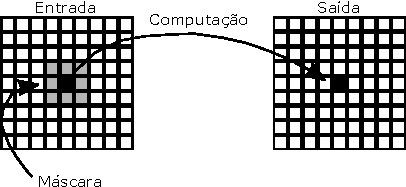
\includegraphics[width=0.7\textwidth]{figs/stencilComp.pdf}
    \caption*{Fonte: desenvolvido pelo autor.}
	\label{fig:stencil}
\end{figure}

Abaixo temos um exemplo do código de uma aplicação baseada no padrão
\textit{stencil}, denominada Jacobi, que tem como o objetivo a
resolução de equações matriciais pelo método iterativo de Jacobi. O número de
iterações é determinado pelo parâmetro \texttt{tsteps} (linha 1). A computação
\textit{stencil} é realizada sobre cada elemento da matriz A, de tamanho N,
utilizando o coeficiente c1 e uma vizinhança de 5 elementos(linha 7). Devido a
sua característica iterativa, existe uma troca de dados entre as matrizes A e B
(linha 8 e 9), pois o resultado da iteração $i$ deve ser utilizado na iteração
$i+1$.

\renewcommand{\lstlistingname}{Código}
\definecolor{lightgray}{rgb}{0.97,0.97,0.97}
\definecolor{lightred}{rgb}{1,0.7,0.7}
\lstdefinelanguage{cc}{
    language     = C++,
    morekeywords = {Array2D, __parallel__, Mask2D, Stencil2D}
}

\lstset{
numbers=left,
stepnumber=1,
numbersep=5pt,
numberstyle=\small\color{black},
basicstyle=\scriptsize\ttfamily,
keywordstyle=\color{blue},
commentstyle=\color{black},
stringstyle=\color{black},
numberstyle=\footnotesize\ttfamily\color{black},
escapeinside={(@}{@)},
% frame=none, %single
tabsize=2,
frame=tb,
xleftmargin=.1\textwidth,
xrightmargin=.1\textwidth,
float,
language=C++, %morecomment=[l][{\color[rgb]{0.1, 0.2, 0.8}}]{},
%aboveskip=0.1in, % space before the caption
%belowskip=0.1in, % space after listing
captionpos=b,
showstringspaces=false,
%belowcaptionskip=1\baselineskip,
breaklines=true,
%moredelim=[l][\color{blue}]{\#pragma},
backgroundcolor=\color{white},
%xleftmargin=.2\textwidth, xrightmargin=.2\textwidth
}

\begin{figure}[bh] % the figure provides the caption
\centering          % which should be centered
\caption*{Exemplo de código da aplicação Jacobi.}
% \begin{tabular}{c}
\begin{lstlisting}[]
void jacobi(int tsteps, int N, float *A, float *B){
    int t, i, j;
    float c1 = 0.2;
    for (t = 0; t < tsteps; t++) {
        for (i = 1; i < N-1; i++) {
            for (j = 1; j < N-1; j++) {
                B(i,j) = c1 * (A(i,j) + A(i,j-1) + A(i,j+1) +
                                          A(i+1,j)+A(i-1,j));
            }
        }
        for (i = 1; i < N-1; i++) {
            for (j = 1; j < N-1; j++) {
                A(i,j) = B(i,j)
            }
        }
    }
}
\end{lstlisting}
% \end{tabular}
\end{figure}



% \todo[inline]{- Adicionar 1 ou 2 parágrafos falando de exemplos de aplicações que usam esse padrão.
% Podes usar o Fur e o Jacobi.}

\section{PSkel}
O PSkel é um \fw de programação em alto nível para o padrão \textit{stencil}, que
oferece suporte à execuções paralelas em arquiteturas heterogêneas incluindo CPU
e GPU. Utilizando uma única interface de programação escrita em C++, o usuário é
responsável por definir o \textit{kernel} principal da computação \textit{stencil},
enquanto o \fw se encarrega de gerar código executável para as diferentes
plataformas paralelas e realizar todo o gerenciamento de memória e transferência
de dados entre dispositivos de forma transparente~\cite{pereira15}. Mais
especificamente, o PSkel traduz as abstrações em código C++ de baixo nível,
compatível com Intel TBB e NVDIA CUDA. Além disso, é utilizado compilação
estática para o particionamnto de tarefas e dados no PSkel.

A API do PSkel possibilita a definição de \textit{templates} para a manipulação
de estruturas $n$-dimensionais, denominadas \texttt{Array} (1 dimensão),
\texttt{Array2D} (2 dimensões) e \texttt{Array3D} (3 dimensões). Além disso, o
\fw provê abstrações para a definição da vizinhança do \textit{stencil} (\texttt{Mask})
e o \textit{kernel} da computação \textit{stencil} (\texttt{stencilKernel()}). O
\texttt{stencilKernel()} é um método a ser implementado pelo usuário que
descreve, especificamente, a computação que será executada para cada célula do
\texttt{Array} de entrada com base nos valores de sua vizinhança (\texttt{Mask}).

Desta forma, o desenvolvedor deverá identificar a dimensão do problema,
construindo estruturas de acordo com os \textit{containers} especificados pelo
\fw; definir o método \texttt{stencilKernel} que descreve a computação executada
sobre os elementos da máscara e do \texttt{Array} de entrada; instanciar um ou
mais objetos \texttt{Stencil} para gerenciar os encapsulamentos, alocação de
memória e chamadas para efetuar a computação determinada pelo
\texttt{stencilKernel}. Mais especificamente, os \textit{containers} são
estruturas que armazenam \texttt{Arrays} para leitura/escrita de dados. Eles são
responsáveis por gerenciar a alocação de memória na \cpu e \gpu.
Por fim, o desenvolvedor irá instanciar a classe de \textit{Runtime} que adota
um padrão \textit{Facade} que efetua a abstração dos detalhes da implementação e
configurações do padrão \textit{stencil}. Essa classe provê os métodos de execução para
os padrões \textit{stencil}, além do particionamento transparente de tarefas e dados
entre \cpu e \gpu.

% \begin{figure}[t]
% \centering
% 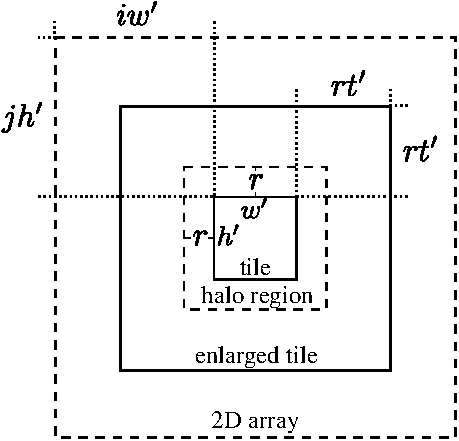
\includegraphics[width=0.3\columnwidth]{figs/tile.pdf}
% \caption{ Diagrama do \textit{tiling} 2D. Um \textit{tile} lógico (linha interna sólida) é contido dentro do Array
%     2D (linha externa pontilhada) com \textit{offsets} verticais e horizontais dado por $j  h^\prime$
%     e $i  w^\prime$. Computar $t^\prime$ consecutivas iterações estêncil no \textit{tile} requer um aumento no
%     \textit{tile} lógico com uma \textit{ghost zone} (área entre a linha interna sólida e a linha externa sólida), que é constituída
%     de regiões \textit{halo} (área entre a linha interna sólida e a linha interna pontilhada).}
% \label{fig:gputile}
% %\vspace{-4em}
% \end{figure}
%
Em uma aplicação \textit{stencil} iterativa, cada iteração utiliza a máscara de
vizinhança (\texttt{Mask}) sobre o \texttt{Array} de entrada para determinar o
valor de cada célula do \texttt{Array} de saída. No exemplo da
Figura~\ref{fig:stencil}, o valor de cada célula do \texttt{Array} de saída é
determinado em função dos valores de cada uma das células vizinhas adjacentes.
Esse processo é realizado para todas as células do \texttt{Array} de entrada,
produzindo um \texttt{Array} de saída da computação \textit{stencil}. Ao final de uma
iteração, o \texttt{Array} de saída será considerado como \texttt{Array} de
entrada para a próxima iteração no caso de uma aplicação \textit{stencil} iterativa.

No código abaixo temos um exemplo da aplicação Jacobi no \fw. Nele temos a
especificação do \texttt{stencilKernel} da aplicação (lina 2 à 7), além das estruturas para
efetuar a computação, como o \texttt{Array} de entrada e saída (linha 11 e 12).
A máscara irá determinar a vizinhança utilizada na computação (linha 14).
Estruturas como \texttt{Array2D}, \texttt{Mask2D}, são exemplos dos
\textit{containers} disponibilizados pelo \fw. A classe de \textit{Runtime} é
determinada pela estrutura \texttt{Stencil2D} (linha 17), onde ao efetuar a chamada para
função \texttt{runIterative} (linha 19), a execução da computação irá iniciar.

% \todo[inline]{Falar mais precisamente o que é feito em cada linha.}

A computação \textit{stencil} (linha 5 e 6) fica mais simplificada, pois os
\texttt{tsteps} e a iteração sobre as matrizes ficam implícitas, sendo
gerenciadas pelo \fw. Os elementos das matrizes são determinados pelos
parâmetros $x$ e $y$ da função \texttt{stencilKernel}. Além disso, o coeficiente
da aplicação Jacobi é passado como parâmetro por uma \texttt{struct} denominada
\texttt{Arguments} (linha 15).

\renewcommand{\lstlistingname}{Código}
\definecolor{lightgray}{rgb}{0.97,0.97,0.97}
\definecolor{lightred}{rgb}{1,0.7,0.7}
\lstdefinelanguage{cc}{
    language     = C++,
    morekeywords = {Array2D, __parallel__, Mask2D, Stencil2D}
}

\lstset{
numbers=left,
stepnumber=1,
numbersep=5pt,
numberstyle=\small\color{black},
basicstyle=\scriptsize\ttfamily,
keywordstyle=\color{blue},
commentstyle=\color{black},
stringstyle=\color{black},
numberstyle=\footnotesize\ttfamily\color{black},
escapeinside={(@}{@)},
frame=tb, %single
tabsize=2,
float,
language=C++, %morecomment=[l][{\color[rgb]{0.1, 0.2, 0.8}}]{},
%aboveskip=0.1in, % space before the caption
%belowskip=0.1in, % space after listing
captionpos=b,
showstringspaces=false,
%belowcaptionskip=1\baselineskip,
%breaklines=true,
%moredelim=[l][\color{blue}]{\#pragma},
backgroundcolor=\color{white},
xleftmargin=.1\textwidth, xrightmargin=.1\textwidth
}

\begin{figure}[thp] % the figure provides the caption
\centering          % which should be centered
\caption*{Exemplo do código da aplicação Jacobi no PSkel.}
% \begin{tabular}{c}

\begin{lstlisting}[]
(@\textcolor{blue}{\textbf{\_\_parallel\_\_}}@) void
stencilKernel((@\textcolor{blue}{\textbf{Array2D}}@)<float> A, (@\textcolor{blue}{\textbf{Array2D}}@)<float> B,
             (@\textcolor{blue}{\textbf{Mask2D}}@)<int> mask, struct Arguments args,
             int x, int y){
    B(x,y) = args.alpha * (A(x,y+1) + A(x,y-1) +
                           A(x+1,y) + A(x-1,y));
 }

void main(){
 /* ... */
 (@\textcolor{blue}{\textbf{Array2D}}@)<float> input(A,M,N);
 (@\textcolor{blue}{\textbf{Array2D}}@)<float> output(B,M,N);
 int neighbors = {{0,1}, {-1,0}, {1,0}, {-1,0}};
 (@\textcolor{blue}{\textbf{Mask2D}}@)<int> mask(4, neighbors);
 struct Arguments args(alpha, beta);
 /* ... */
 (@\textcolor{blue}{\textbf{Stencil2D}}@)<Array2D<float>, Mask2D<int>, Arguments>
             jacobi(A,B,args);
 jacobi.runIterative(device::GPU, timesteps, 1.0);
 /* ... */
}
\end{lstlisting}
% \end{tabular}
\end{figure}


